\section{Case study}
\begin{figure}[htbp]
  \centering
  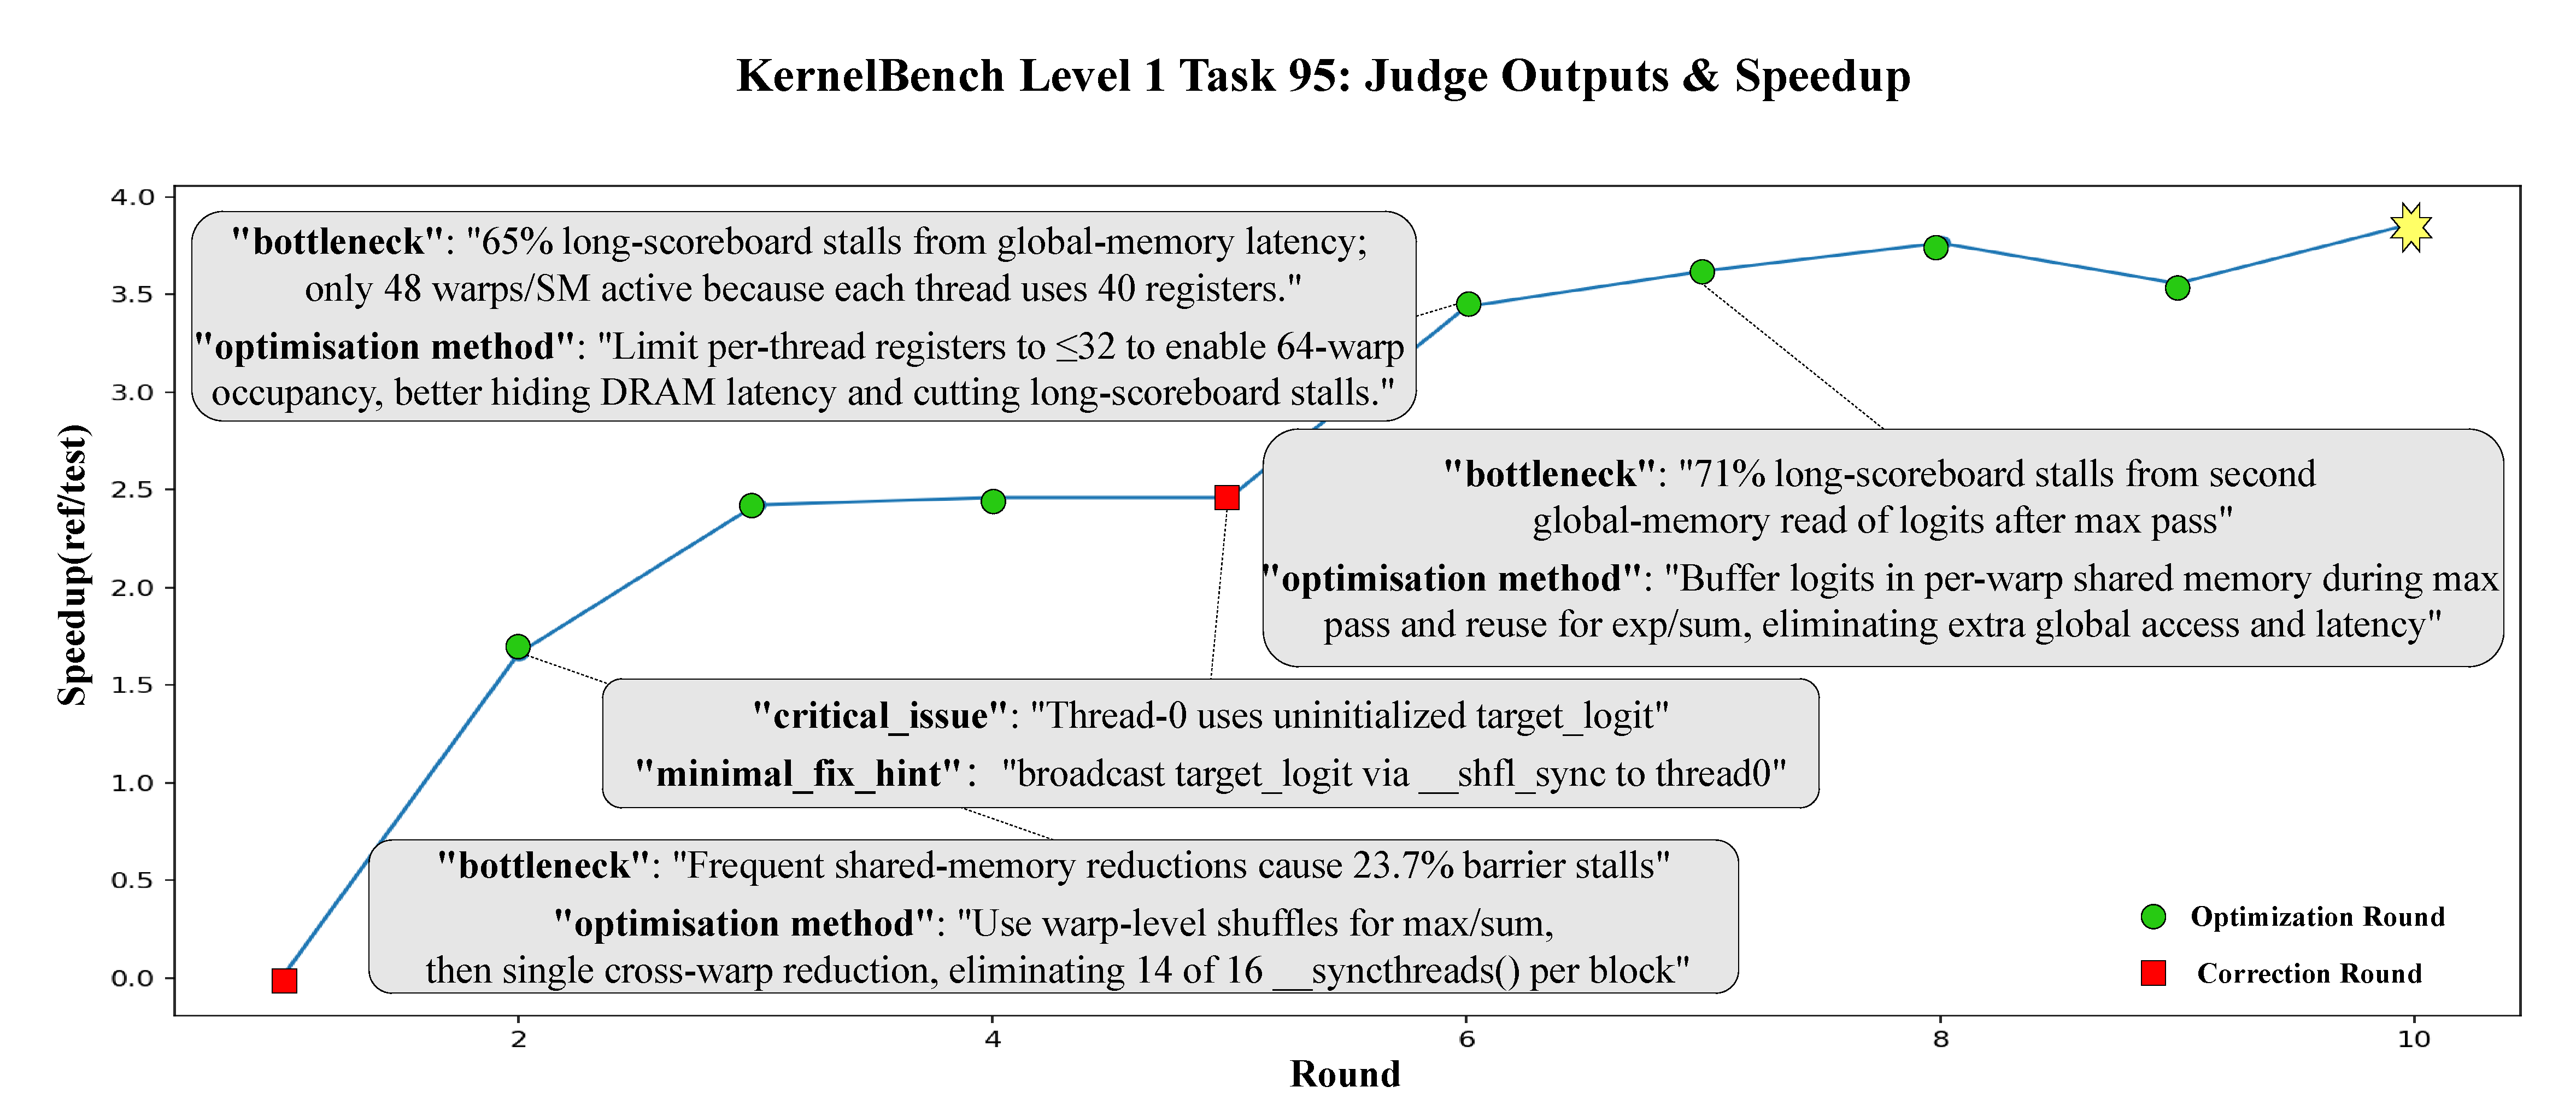
\includegraphics[width=1.0\linewidth]{pic/case_study_v1.pdf}
  \caption{Illustration of the Judge’s outputs—bottleneck diagnoses and optimization suggestions—on KernelBench Level-1 Task 95 (CrossEntropyLoss), as well as the correspondi speedup across rounds (green = optimization, red = correction).}
  \label{fig:good_case}
\end{figure}

In this section, we present a case study on a single task to illustrate how the Judge diagnoses issues and recommends optimizations. Figure~\ref{fig:good_case} depicts the 10-round refinement process of \agentname~ on task \texttt{95\_CrossEntropyLoss}. We highlight four representative rounds—three optimization rounds and one repair round—to demonstrate how the Judge leverages hardware feedback from NCU to provide targeted optimization or bug-fix suggestions.


In round 2, which is an optimization round, the Judge notices that 23.7\% of active warps are stalled due to barrier-type dependencies, which means roughly one quarter of potential issue opportunities are blocked by synchronization. According to this, the Judge recommended replacing the original shared-memory reduction that required multiple block-level synchronizations with a warp-level shuffle reduction, giving below suggestion as prompt for coder: use warp-level shuffles in the max and sum phases, then perform a single cross-warp combine, reducing \texttt{\_\_syncthreads()} per block from 16 to 2 (a reduction of 14). After applying this change, performance improved from \(\mathbf{1.66\times}\) to \(\mathbf{2.42\times}\), with barrier stalls reduced and instruction-issue efficiency increased.

In round 5, it is a correction round. The previous round fails a numerical check with the following error: ``Outputs are not close, indicating a result mismatch". The Judge diagnosed the root cause as an uninitialized target\_logit in thread 0 (“Thread-0 uses uninitialized target\_logit”), which means the variable target\_logit is not updated to thread 0, leading wrong computing results. Accordingly, the Judge gave the minimal fix suggestion, broadcast \texttt{target\_logit} via \texttt{\_shfl\_sync} to thread 0. After applying the fix, the numerical issue disappeared.

In rounds 6 \& 7 (both optimization rounds), the Judge continues to track smsp\_warp\_issue \_stalled\_long\_scoreboard\_per\_warp\_active.pct. 
In round~6, this metric is about \(65\%\), primarily reflecting long-scoreboard stalls caused by global-memory latency. Per-thread register usage is high, resulting in limited occupancy (only \(\sim48\) active warps/SM) and insufficient latency hiding. 
The recommendation is to reduce per-thread registers to raise concurrency to \(\sim64\) warps/SM and thereby lower the long-scoreboard share. 
In round~7, the metric rises to about \(71\%\), rooted in a second global read of logits after the max pass. 
The Judge therefore advises buffering logits in per-warp shared memory during the max pass and reusing them in the exp\/sum phase, eliminating the redundant global memory access. 
Together, these strategies reduce global memory access, significantly cut long-scoreboard stalls, improve issue efficiency and throughput; after these two rounds, the speedup increases from \(3.436\times\) to \(3.762\times\).

This task demonstrates our \agentname's stability and expert-like workflow: first analyzing bottlenecks from hardware feedback, then deriving the corresponding optimization strategy.

\section{Supplement Observations}

\noindent{\bf Observations in CUDA-L1 results.} We carefully examined the kernel outputs reported by CUDA-L1 (see Appendix~\ref{app:cuda-l1}) and identified an interesting phenomenon that we term \emph{"fake kernels".}
These kernels, while reported as performant, often contain no actual CUDA code. Instead, they rely on \texttt{try-except} constructs and fall back to PyTorch’s official implementations to solve the task.
This observation highlights a fundamental challenge in evaluating LLM-generated CUDA kernels. To avoid this issue, we have manually checked all kernels in our experiments.


\section{Conclusion}
We presented \agentname, a training-free multi-agent framework for CUDA kernel generation and optimization.
The framework imitates the iterative workflow of human experts, explicitly incorporating hardware feedback to guide targeted kernel refinement rather than blind exploration. On the KernelBench benchmark, \agentname~achieves highest correctness rate and significant performance gains compared with all existing method, while also demonstrating robustness across diverse GPU architectures and base LLMs 
Moreover, its performance scales effectively with the number of refinement rounds.
Finally, thanks to its low API and time cost, \agentname~provides a practical and efficient solution for automated CUDA kernel development.

\newpage